% !TEX program = xelatex
\documentclass[10pt,twocolumn]{article}

\usepackage[margin=0.75in]{geometry}
\usepackage[UTF8,scheme=plain]{ctex}
\usepackage{times}
\usepackage{microtype}
\usepackage{amsmath,amssymb}
\usepackage{booktabs}
\usepackage{graphicx}
\usepackage{multirow}
\usepackage{xcolor}
\usepackage{hyperref}
\usepackage{enumitem}
\usepackage{caption}

\hypersetup{
  colorlinks=true,
  linkcolor=blue!60!black,
  citecolor=blue!60!black,
  urlcolor=blue!60!black
}

\setlength{\columnsep}{0.25in}
\captionsetup{font=small,labelfont=bf}

\title{\textbf{When Do Synthetic Queries Mislead Retriever Selection?\\
Selection Reversal, Candidate-Set Abstention, and Eligibility-Condition Preservation in Chinese Insurance Retrieval}}

\author{
  \textbf{Shunchi Wang}\thanks{Correspondence to: \texttt{wangshunchi@example.com}. Reproducible code, group-disjoint splits, traceable policy clause tables, and blinded annotation packages are available at \url{https://github.com/jakelihua/chinese-insurance-rag-benchmark}.} \\
  Independent Researcher
}

\date{}

\begin{document}
\maketitle

\begin{abstract}
When cold-starting a vertical-domain retrieval-augmented generation (RAG) system, engineering teams routinely rely on rule-based proxies or large language model (LLM) synthetic queries to benchmark candidate retrievers before real user logs are available. Yet a fundamental decision-theoretic question remains under-explored: \emph{when does ranking retrievers on synthetic queries reverse the true winner on real user queries, and why do format-valid synthetic queries silently corrupt domain-specific eligibility conditions across model scales?}

We investigate this question through a three-round diagnostic study on Chinese insurance retrieval and clause-level underwriting/claims eligibility verification across a three-tier model hierarchy (\texttt{Qwen2.5-1.5B-Instruct}, \texttt{Qwen-Plus}, and \texttt{Qwen-Max}). In \textbf{Round~1}, we curate $3{,}746$ real insurance QA pairs partitioned into $3{,}725$ connected groups to prevent duplicate-answer leakage, evaluating candidate retrievers across $2{,}994$ held-out real queries. In \textbf{Round~2}, we uncover a statistically significant \textbf{retriever selection reversal} that persists across model scales: both local \texttt{Qwen2.5-1.5B-Instruct} ($N=249$) and cloud \texttt{Qwen-Plus} ($N=179$) synthetic benchmarks rank hybrid fusion (\texttt{rrf\_bm25\_bge}) first under both \texttt{zero\_shot} ($0.5647$ and $0.7371$) and \texttt{few\_shot\_3} ($0.4124$ and $0.6813$), whereas held-out real queries significantly favor pure dense retrieval (\texttt{bge\_small\_zh}, $0.5216$ vs.\ $0.5030$; paired $\Delta = +0.0187$, 95\% bootstrap CI $[+0.0080, +0.0300]$). Surface-feature importance weighting fails to rescue this bias ($0\%$ optimal selection rate), whereas a paired-bootstrap \textbf{Candidate-Set Abstention} policy eliminates confident wrong selection at small calibration budgets ($B=25$: from $60\text{--}100\%$ down to $0.0\%$) while retaining $100\%$ coverage of the true oracle winner. In \textbf{Round~3}, using $80$ controlled clause-grounded cases with single-field counterexample witnesses and $120$ paired LLM rewrites across five official insurance policy wordings ($3$ model tiers $\times 40$ jobs), we show that $100\%$ ($120/120$) of generated queries pass syntactic format checks (\texttt{format\_valid}). Scaling from \texttt{1.5B} to \texttt{Qwen-Plus} and flagship \texttt{Qwen-Max} eliminates numeric value hallucinations ($15\% \rightarrow 0\%$) but \emph{fails to prevent pragmatic condition omission} under ordinary conversational prompting (\texttt{ordinary\_style}), yielding only $0\%\text{--}20\%$ standalone rule-decision preservation. Explicitly constraining eligibility slots (\texttt{condition\_prompt}) restores standalone rule-decision preservation to $95\%$ on \texttt{1.5B}/\texttt{Qwen-Plus} and \textbf{$100\%$ ($20/20$)} on \texttt{Qwen-Max}, while lifting top-1 clause retrieval to $95\%\text{--}100\%$.
\end{abstract}

\section{Introduction}
Deploying retrieval-augmented generation (RAG) in regulated verticals such as insurance, healthcare, and consumer finance requires selecting an effective retriever---choosing among character/lexical matching, dense bi-encoders, or hybrid reciprocal rank fusion (RRF)---frequently before large-scale production query logs exist. Standard practice in both academic benchmarks \cite{dai2023promptagator,jeronymo2023inparsv2} and automated RAG evaluation frameworks such as ARES \cite{saadfalcon2024ares} and RAGAs \cite{es2024ragas} is to prompt an instruction-tuned LLM to synthesize user queries from corpus passages, evaluate candidate retrievers on those synthetic queries, and deploy the top-ranked retriever.

While recent studies have examined how well synthetic test collections correlate with real system rankings at the macro level \cite{rahmani2024syndl,boyd2025reckoning}, practical vertical-domain engineering faces two acute failure modes that aggregate rank correlations obscure:
\begin{enumerate}[leftmargin=*,nosep]
  \item \textbf{Top-1 Retriever Selection Reversal}: If a generative model systematically copies lexical terminology from source passages, hybrid retrievers that combine BM25 with dense embeddings gain an artificial lexical boost on synthetic benchmarks. When real users ask colloquial, vocabulary-mismatched questions, the lexical component injects false-positive noise into top ranks, reversing the true winner between dense and hybrid retrieval.
  \item \textbf{Silent Erosion of Eligibility Conditions}: In insurance claims and underwriting, whether a claim is covered (\texttt{WAIT\_NOT\_EXCLUDED}) or denied (\texttt{WAIT\_EXCLUDED}) hinges on fine-grained conditions: policy waiting periods (7 vs.\ 25 vs.\ 30 vs.\ 90 days), accidental injury vs.\ sickness etiology, first-time vs.\ renewal enrollment, and explicit waiver approvals. When an LLM rewrites a structured case into a ``natural'' customer question, it passes surface validity filters (question marks, length, character overlap) 100\% of the time while silently dropping or mutating the exact condition that determines the legal outcome.
\end{enumerate}

In this paper, we present a controlled, three-round empirical study of these failure modes in Chinese insurance retrieval across local edge (\texttt{Qwen2.5-1.5B-Instruct}), mid-tier production (\texttt{Qwen-Plus}), and frontier flagship (\texttt{Qwen-Max}) models. Our contributions are fourfold:
\begin{itemize}[leftmargin=*,nosep]
  \item \textbf{Group-Disjoint Benchmark \& Proxy Baseline (Round~1)}: We construct a group-disjoint Chinese insurance retrieval split ($3{,}746$ answers, $3{,}725$ connected groups, $2{,}994$ held-out real test queries) that prevents duplicate-answer leakage, quantifying the selection regret of naive surface copy proxies ($0.1090$ MRR@10 regret) and small real calibration sets.
  \item \textbf{Cross-Scale Demonstration of LLM Selection Reversal (Round~2)}: We show that both \texttt{Qwen2.5-1.5B-Instruct} ($N=249$) and \texttt{Qwen-Plus} ($N=179$) rank \texttt{rrf\_bm25\_bge} first under both \texttt{zero\_shot} and \texttt{few\_shot\_3} synthetic benchmarks, whereas held-out real queries significantly favor pure dense retrieval (\texttt{bge\_small\_zh}, paired $\Delta = +0.0187$, 95\% CI $[+0.0080, +0.0300]$).
  \item \textbf{Negative Result for Surface Reweighting \& Candidate-Set Abstention}: We demonstrate that importance weighting over four surface statistics fails to correct selection reversal ($0\%$ optimal selection rate), because the bias is structural (conditional lexical copying $P(q \mid d)$) rather than a marginal covariate shift. In contrast, a paired-bootstrap \textbf{Candidate-Set Abstention} policy reduces confident wrong selection at budget $B=25$ from $60\text{--}100\%$ to $0.0\%$ while preserving $100\%$ optimal winner coverage.
  \item \textbf{Multi-Scale Condition Drift \& Slot-Preserving Generation (Round~3)}: Across five official insurance policy wordings ($80$ controlled cases and $120$ paired LLM rewrites across \texttt{1.5B}, \texttt{Qwen-Plus}, and \texttt{Qwen-Max}), we decouple syntactic validity ($120/120$ pass \texttt{format\_valid}) from semantic condition preservation. We show that scaling up model capacity eliminates value hallucinations ($15\% \rightarrow 0\%$) but does \emph{not} prevent pragmatic slot omission under \texttt{ordinary\_style} ($0\%\text{--}20\%$ standalone decision preservation), whereas \texttt{condition\_prompt} achieves $95\%$ on \texttt{1.5B}/\texttt{Qwen-Plus} and $100\%$ ($20/20$) on \texttt{Qwen-Max}.
\end{itemize}

\section{Related Work}
\paragraph{Synthetic Queries for IR and RAG Evaluation.}
Promptagator \cite{dai2023promptagator} and InPars-v2 \cite{jeronymo2023inparsv2} demonstrated that LLM-generated synthetic queries can effectively train dense retrievers. Automated RAG evaluation suites including ARES \cite{saadfalcon2024ares} and RAGAs \cite{es2024ragas} further use synthetic queries for zero-human-label system benchmarking. More recently, Rahmani et al.\ \cite{rahmani2024syndl} and Boyd et al.\ \cite{boyd2025reckoning} cautioned that synthetic evaluation sets exhibit model-specific biases. Our work complements these macro-level studies by pinpointing a concrete \emph{dense vs.\ hybrid selection reversal} driven by lexical copy inflation across model scales and showing how to hedge against it via candidate-set abstention.

\paragraph{Statistical Calibration and Abstention.}
Prediction-Powered Inference (PPI) \cite{angelopoulos2023prediction} and ARES \cite{saadfalcon2024ares} combine large synthetic sets with small gold calibration samples to form unbiased confidence intervals. We extend this perspective to the \emph{discrete model-selection problem} under tight annotation budgets ($B \in [25, 200]$), showing that returning a statistically indistinguishable candidate set when bootstrap confidence intervals overlap zero prevents premature lock-in to a suboptimal retriever.

\paragraph{Domain-Specific Insurance QA.}
InsuranceQA \cite{feng2020insuranceqa} established answer selection in insurance domains using general FAQ queries. However, general FAQ retrieval does not test whether fine-grained policy eligibility conditions (waiting periods, accident exceptions, renewal waivers) survive query synthesis or remain decidable against real policy clauses. Our Round~3 benchmark bridges retrieval evaluation and deterministic rule verification on official Chinese insurance clauses.

\section{Round 1: Group-Disjoint Retrieval Benchmark \& Proxy Diagnostics}

\subsection{Dataset Construction and Leakage Prevention}
Real-world insurance FAQ datasets frequently contain near-duplicate or verbatim answers shared across multiple paraphrased user questions. A naive random train/test split places identical answer passages in both calibration and test pools, inflating lexical retrieval scores.

Starting from the corpus derived from insuranceQA-zh, we extract $3{,}746$ unique answer documents after normalizing whitespace and deduplicating exact text matches. We then construct an undirected graph over all QA pairs that share normalized question or answer strings and compute connected components via Union-Find, yielding $3{,}725$ disjoint groups. We partition groups strictly at the component level into:
\begin{itemize}[leftmargin=*,nosep]
  \item \textbf{Calibration Pool}: $750$ queries across $745$ groups (used for few-shot exemplars and low-budget real calibration sampling).
  \item \textbf{Held-Out Real Test Set}: $2{,}994$ queries across $2{,}980$ groups (used as the oracle evaluation benchmark).
\end{itemize}

\subsection{Candidate Retrievers and Proxy Regimes}
We evaluate four core retrieval architectures spanning lexical, dense, and hybrid paradigms:
\begin{enumerate}[leftmargin=*,nosep]
  \item \texttt{bm25\_char2}: Okapi BM25 ($k_1=1.5, b=0.75$) over overlapping Chinese character bigrams.
  \item \texttt{tfidf\_char3\_5}: Sublinear TF-IDF cosine similarity over character $3\text{--}5$-grams.
  \item \texttt{bge\_small\_zh}: Dense bi-encoder retrieval using \texttt{BAAI/bge-small-zh-v1.5} (512-dim normalized embeddings).
  \item \texttt{rrf\_bm25\_bge}: Reciprocal Rank Fusion ($k=60$) combining top-100 rankings from \texttt{bm25\_char2} and \texttt{bge\_small\_zh}.
\end{enumerate}

In Round~1, we compare held-out real queries against two non-LLM heuristic proxies: \texttt{synth\_keyword} (extracting top TF-IDF domain keywords wrapped in insurance question templates) and \texttt{synth\_SnippetCopy} (a diagnostic stress test extracting the leading sentence fragment of the answer).

\begin{table}[t]
\centering
\small
\caption{Round~1 full-sample retrieval evaluation ($N=2{,}994$ held-out real test queries vs.\ heuristic proxies).}
\label{tab:round1}
\resizebox{\columnwidth}{!}{
\begin{tabular}{lcccc}
\toprule
\textbf{Query Regime} & \textbf{Metric} & \texttt{bm25\_c2} & \texttt{tfidf\_c3\_5} & \textbf{Winner} \\
\midrule
Held-Out Real & MRR@10 & \textbf{0.4907} & 0.3817 & \texttt{bm25} \\
Held-Out Real & Recall@1 & \textbf{0.4606} & 0.3490 & \texttt{bm25} \\
\midrule
\texttt{synth\_keyword} & MRR@10 & \textbf{0.9335} & 0.8732 & \texttt{bm25} \\
\texttt{synth\_SnippetCopy} & MRR@10 & 0.9462 & \textbf{0.9502} & \texttt{tfidf} \\
\bottomrule
\end{tabular}
}
\end{table}

\begin{figure}[t]
  \centering
  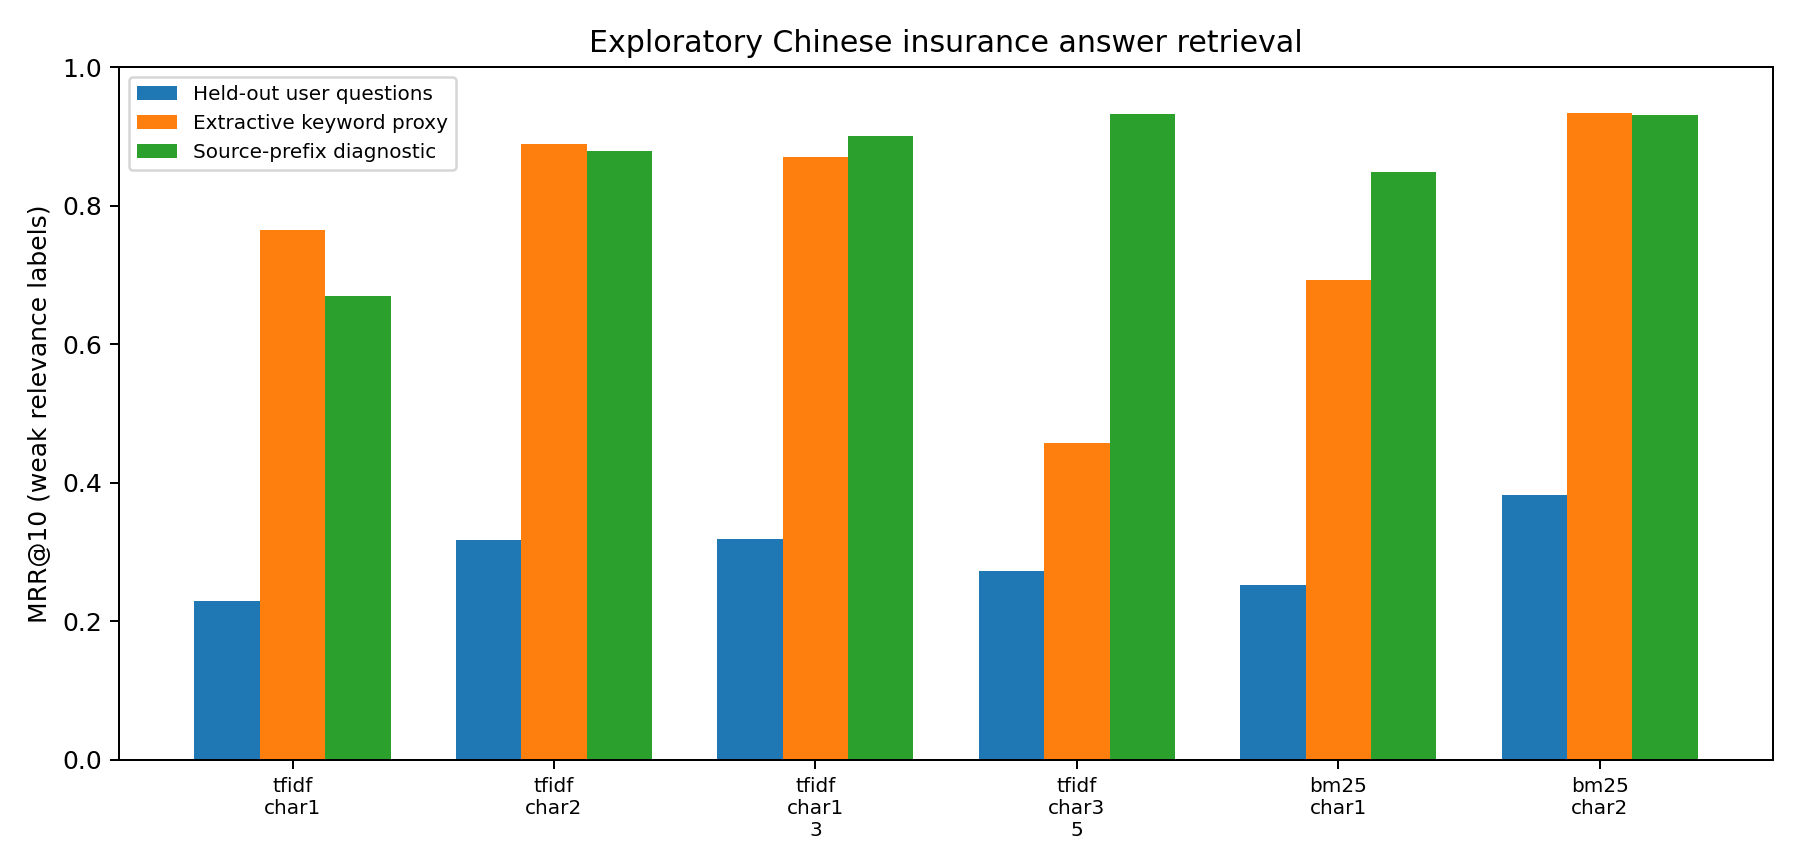
\includegraphics[width=\columnwidth]{figures/retrieval_comparison.png}
  \caption{Round~1 comparison of retriever performance across held-out real queries, keyword proxy queries, and snippet-copy diagnostic queries.}
  \label{fig:round1}
\end{figure}

\subsection{Round 1 Findings}
As shown in Table~\ref{tab:round1} and Figure~\ref{fig:round1}, on all $2{,}994$ held-out real queries, \texttt{bm25\_char2} achieves $\text{MRR@10}=0.4907$ versus $0.3817$ for \texttt{tfidf\_char3\_5}. While \texttt{synth\_keyword} preserves the pairwise ordering, \texttt{synth\_SnippetCopy} inflates longer character $n$-gram overlap and erroneously selects \texttt{tfidf\_char3\_5}, incurring a true deployment regret of $0.1090$ MRR@10. Furthermore, across $200$ repeated subsampling trials per budget $B \in \{25, 50, 100, 200\}$, sampling just $B \ge 50$ real calibration queries achieves a $100\%$ optimal selection rate with zero regret.

\section{Round 2: LLM Synthetic Queries, Selection Reversal, and Abstention}

\subsection{Multi-Scale Experimental Setup}
Heuristic proxies cannot represent modern LLM query synthesis. In Round~2, we evaluate two distinct model scales: a locally deployed 1.5B edge model (\texttt{Qwen2.5-1.5B-Instruct} in deterministic \texttt{float32/eager} mode, $N=249$ shared valid sources) and a production cloud model (\texttt{Qwen-Plus} at $\text{temperature}=0$, $N=179$ shared valid sources) under two prompting strategies:
\begin{itemize}[leftmargin=*,nosep]
  \item \texttt{zero\_shot}: Prompting the LLM with only the target insurance answer passage to generate a single customer question.
  \item \texttt{few\_shot\_3}: Conditioning the prompt on three real question--answer exemplars drawn strictly from the disjoint calibration pool before presenting the target passage.
\end{itemize}

\begin{table*}[t]
\centering
\small
\caption{Round~2 retriever evaluation across held-out real queries and multi-scale LLM synthetic benchmarks (\texttt{Qwen2.5-1.5B-Instruct} and \texttt{Qwen-Plus}). Across both model scales and both prompting regimes (\texttt{zero\_shot} and \texttt{few\_shot\_3}), synthetic benchmarks select \texttt{rrf\_bm25\_bge}, reversing the true held-out winner \texttt{bge\_small\_zh} (paired $\Delta = +0.0187$, 95\% bootstrap CI $[+0.0080, +0.0300]$).}
\label{tab:round2}
\resizebox{\textwidth}{!}{
\begin{tabular}{llccccc}
\toprule
\textbf{Query Regime / Generator} & \textbf{Metric} & \texttt{bm25\_char2} & \texttt{tfidf\_char3\_5} & \texttt{bge\_small\_zh} & \texttt{rrf\_bm25\_bge} & \textbf{Selected Winner} \\
\midrule
Held-Out Real Test ($N=2{,}994$) & MRR@10 & 0.3817 & 0.2727 & \textbf{0.5216} & 0.5030 & \textbf{\texttt{bge\_small\_zh} (True Winner)} \\
Held-Out Real Matched ($N=249$) & MRR@10 & 0.4539 & 0.3408 & \textbf{0.5216} & 0.5030 & \textbf{\texttt{bge\_small\_zh} (True Winner)} \\
\midrule
\texttt{Qwen2.5-1.5B} \texttt{zero\_shot} ($N=249$) & MRR@10 & 0.4910 & 0.3554 & 0.5177 & \textbf{0.5647} & \texttt{rrf\_bm25\_bge} (Reversed, $\Delta=-0.0470$) \\
\texttt{Qwen2.5-1.5B} \texttt{few\_shot\_3} ($N=249$) & MRR@10 & 0.3694 & 0.2330 & 0.3910 & \textbf{0.4124} & \texttt{rrf\_bm25\_bge} (Reversed, $\Delta=-0.0214$) \\
\midrule
\texttt{Qwen-Plus} \texttt{zero\_shot} ($N=179$) & MRR@10 & 0.6528 & 0.4553 & 0.7005 & \textbf{0.7371} & \texttt{rrf\_bm25\_bge} (Reversed, $\Delta=-0.0366$) \\
\texttt{Qwen-Plus} \texttt{few\_shot\_3} ($N=179$) & MRR@10 & 0.5747 & 0.3832 & 0.6794 & \textbf{0.6813} & \texttt{rrf\_bm25\_bge} (Reversed, $\Delta=-0.0019$) \\
\bottomrule
\end{tabular}
}
\end{table*}

\begin{figure}[t]
  \centering
  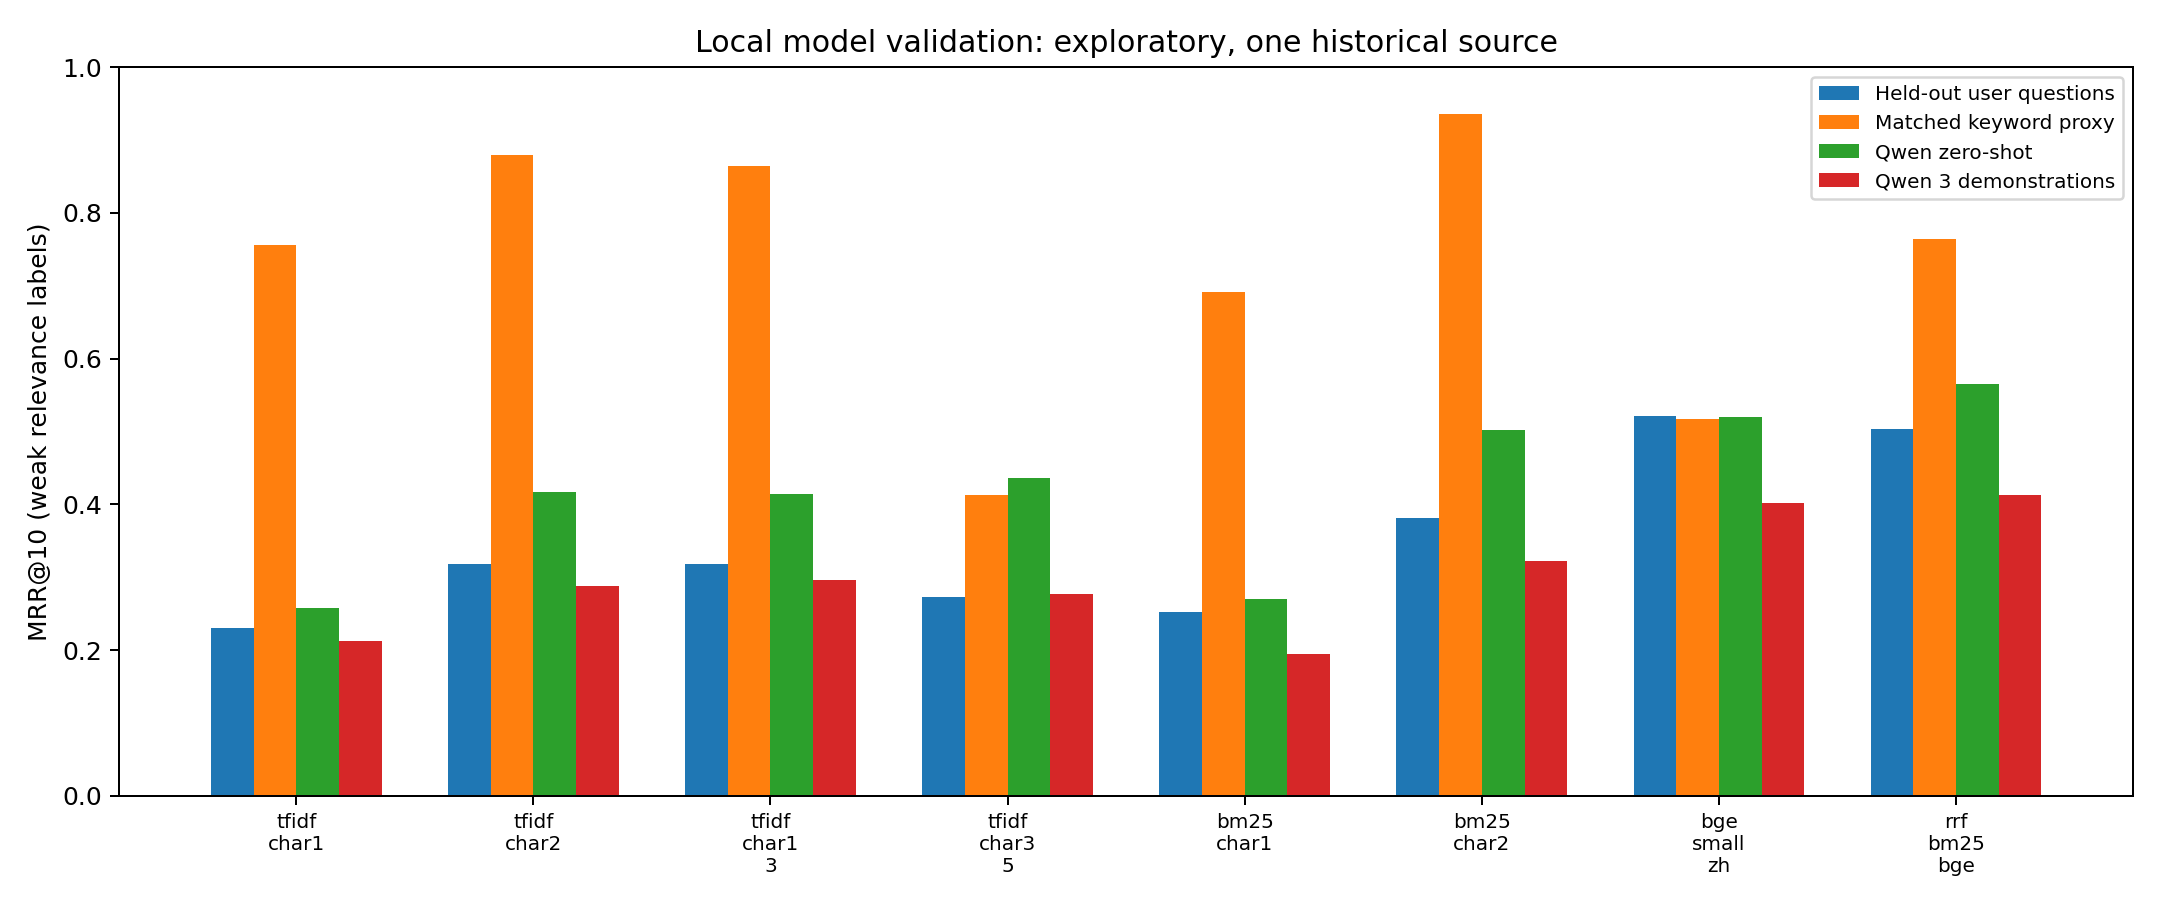
\includegraphics[width=\columnwidth]{figures/comparison.png}
  \caption{Round~2 retriever selection reversal across real held-out queries and LLM synthetic query regimes ($N=249$ shared sources).}
  \label{fig:round2}
\end{figure}

\subsection{Mechanism of Retriever Selection Reversal Across Scales}
Table~\ref{tab:round2} and Figure~\ref{fig:round2} reveal that \textbf{retriever selection reversal is not merely an artifact of a small 1.5B model}:
\begin{enumerate}[leftmargin=*,nosep]
  \item \textbf{True Held-Out Winner}: On real user queries, pure dense retrieval (\texttt{bge\_small\_zh}) achieves the highest performance ($\text{MRR@10}=0.5216$), outperforming hybrid fusion (\texttt{rrf\_bm25\_bge}, $0.5030$) by a paired difference of $+0.0187$ (1,000-resample paired bootstrap 95\% CI: $[+0.0080, +0.0300]$, excluding zero). Because real users ask short ($11.50$ chars), colloquial questions with low character bigram overlap ($0.0713$), lexical \texttt{bm25\_char2} is weak ($0.3817$ overall, $0.4539$ matched) and fusing it via RRF dilutes the top ranks of \texttt{bge\_small\_zh}.
  \item \textbf{Persistent Reversal under \texttt{zero\_shot}}: On \texttt{Qwen2.5-1.5B}, \texttt{zero\_shot} increases bigram overlap by $68\%$ ($0.1197$), boosting \texttt{rrf\_bm25\_bge} to $0.5647$ over \texttt{bge\_small\_zh} ($0.5177$). Scaling up to \texttt{Qwen-Plus} produces even stronger domain-terminology alignment under \texttt{zero\_shot}: \texttt{bm25\_char2} jumps to $0.6528$, driving \texttt{rrf\_bm25\_bge} ($0.7371$) to beat \texttt{bge\_small\_zh} ($0.7005$) by $+0.0366$ MRR@10.
  \item \textbf{Effect of \texttt{few\_shot\_3} Across Scales}: On \texttt{Qwen2.5-1.5B}, conditioning on 3 calibration exemplars suppresses surface copying (bigram overlap drops to $0.0724$) but induces semantic drift ($\text{MRR@10}=0.3910$), still selecting \texttt{rrf\_bm25\_bge} ($0.4124$). On the larger \texttt{Qwen-Plus} model, \texttt{few\_shot\_3} avoids semantic drift ($\text{MRR@10}=0.6794$) and narrows the reversal gap from $-0.0366$ to $-0.0019$, \emph{yet \texttt{rrf\_bm25\_bge} ($0.6813$) still edges out \texttt{bge\_small\_zh} ($0.6794$) under naive point selection}.
\end{enumerate}

\subsection{Why Surface Reweighting Fails and Candidate-Set Abstention Works}
Computing importance weights over standardized query length, bigram overlap, trigram overlap, and longest common substring ratio relative to calibration queries yields a \textbf{$0.0\%$ optimal selection rate} across all budgets $B \in \{25, 50, 100, 200\}$ (mean regret $0.0187$), because the bias stems from the passage-conditioned generation process $P(q \mid d)$ rather than marginal query covariates.

To prevent confident wrong commitments, we apply \textbf{Candidate-Set Abstention}: given a query sample of size $B$, we identify the empirical leader $\hat{r}^*$ and run $M=200$ paired bootstrap resamples. Any retriever $r$ whose 95\% paired difference confidence interval against $\hat{r}^*$ overlaps zero is retained in $\mathcal{C}_B$. If $|\mathcal{C}_B| > 1$, the selector abstains from a single point commitment and returns $\mathcal{C}_B$.

\begin{table}[t]
\centering
\small
\caption{Confident Wrong Selection Rate (Commit Error $\downarrow$) and Optimal Winner Coverage ($\uparrow$) under Point Selection vs.\ Candidate-Set Abstention across $50$ trials per budget $B$.}
\label{tab:abstention}
\resizebox{\columnwidth}{!}{
\begin{tabular}{llcccc}
\toprule
\textbf{Strategy} & \textbf{Metric} & $B=25$ & $B=50$ & $B=100$ & $B=200$ \\
\midrule
\texttt{real\_only} (Point) & Commit Error $\downarrow$ & 60.0\% & 52.0\% & 28.0\% & 4.0\% \\
\texttt{zero\_shot} (Point) & Commit Error $\downarrow$ & 100.0\% & 100.0\% & 100.0\% & 100.0\% \\
\texttt{few\_shot\_3} (Point) & Commit Error $\downarrow$ & 80.0\% & 92.0\% & 98.0\% & 100.0\% \\
\midrule
\textbf{\texttt{real\_only} (Abstain)} & \textbf{Commit Error} $\downarrow$ & \textbf{0.0\%} & \textbf{0.0\%} & \textbf{0.0\%} & \textbf{0.0\%} \\
\textbf{\texttt{real\_only} (Abstain)} & \textbf{Opt.\ Coverage} $\uparrow$ & \textbf{100.0\%} & \textbf{100.0\%} & \textbf{100.0\%} & \textbf{100.0\%} \\
\textbf{\texttt{real\_only} (Abstain)} & Mean Set Size & 2.60 & 2.12 & 1.88 & 1.80 \\
\midrule
\textbf{\texttt{few\_shot\_3} (Abstain)} & \textbf{Commit Error} $\downarrow$ & \textbf{0.0\%} & 2.0\% & 0.0\% & 0.0\% \\
\textbf{\texttt{few\_shot\_3} (Abstain)} & \textbf{Opt.\ Coverage} $\uparrow$ & \textbf{100.0\%} & 98.0\% & 100.0\% & 98.0\% \\
\bottomrule
\end{tabular}
}
\end{table}

As shown in Table~\ref{tab:abstention}, Candidate-Set Abstention eliminates confident wrong commitments at $B=25$ (\textbf{$0.0\%$ commit error}) while narrowing the 4 core retrievers down to an average candidate set of $2.12\text{--}2.60$ retrievers with $100\%$ coverage of the true winner (\texttt{bge\_small\_zh}).

\section{Round 3: Clause-Grounded Eligibility-Condition Preservation Across Model Scales}

\subsection{Traceable Insurance Clauses and Counterexample Witnesses}
Even if a retriever fetches the right policy document, an insurance RAG benchmark is invalid if synthetic queries alter the facts that determine coverage. We curate five official Chinese insurance policy wordings spanning group medical, inpatient, and internet outpatient scenarios (Table~\ref{tab:clauses}).

\begin{table*}[t]
\centering
\small
\caption{Five traceable official Chinese insurance policy clauses used in Round~3 condition-sensitivity evaluation.}
\label{tab:clauses}
\resizebox{\textwidth}{!}{
\begin{tabular}{llp{11.5cm}}
\toprule
\textbf{Policy ID} & \textbf{Wait Period} & \textbf{Key Eligibility / Exception Rules} \\
\midrule
\texttt{pa\_p0781} & 90 days & Ping An Group Medical (Plan B): 90d wait for specified/mild diseases; accidental injury waives wait. \\
\texttt{pa\_h865} & 30 days & Ping An Employee \& Dependent Inpatient: 30d wait; accidental injury or approved waiver exempts wait. \\
\texttt{cpic\_86017} & 7--25 days & CPIC Internet Outpatient (Plan C): plan-specific wait (7/15/25d); renewal with insurer approval waives wait. \\
\texttt{cpic\_82859} & 30 days & CPIC Personal 1-Year Inpatient (Plan E): 30d wait; accidental injury or approved renewal waives wait. \\
\texttt{tk\_group\_2018} & 30 days & Taikang Group Inpatient (2018): 30d wait; accidental injury waives wait; psychiatric conditions excluded. \\
\bottomrule
\end{tabular}
}
\end{table*}

We construct $20$ seed scenarios expanded into $80$ controlled cases across four variants (\texttt{complete}, \texttt{surface}, \texttt{missing\_critical}, and \texttt{counterfactual}). Every seed is paired with a \textbf{single-field counterexample witness}: flipping one pivotal field (e.g., changing \texttt{policy\_day} from day~20 to day~45, changing \texttt{cause} from sickness to accident, or switching \texttt{plan\_wait\_days} from 7d to 25d) strictly flips the deterministic rule outcome between \texttt{WAIT\_EXCLUDED} and \texttt{WAIT\_NOT\_EXCLUDED} ($100\%$ flip rate across all counterexamples).

\subsection{Multi-Scale Paired LLM Rewriting (\texttt{1.5B} vs.\ \texttt{Qwen-Plus} vs.\ \texttt{Qwen-Max})}
To test whether scaling up LLM capability automatically solves eligibility-condition drift, we evaluate all $20$ seed cases across three model tiers---\texttt{Qwen2.5-1.5B-Instruct} (local edge), \texttt{Qwen-Plus} (production cloud), and \texttt{Qwen-Max} (flagship frontier)---generating $3 \times 40 = 120$ paired rewrites under two prompting protocols:
\begin{itemize}[leftmargin=*,nosep]
  \item \texttt{ordinary\_style}: Instructs the LLM to rewrite the structured scenario into a short, natural customer question preserving original intent.
  \item \texttt{condition\_prompt}: Instructs the LLM to rewrite the question naturally while explicitly preserving all required slots (product full name, first/renewal enrollment, effective day, sickness/accident cause, plan waiting days, and waiver approval status).
\end{itemize}

\begin{table*}[t]
\centering
\small
\caption{Round~3 multi-scale condition preservation and retrieval impact across $120$ paired LLM rewrites ($3$ model tiers $\times 20$ seeds $\times 2$ prompt styles). Scaling from \texttt{1.5B} to \texttt{Qwen-Plus} and \texttt{Qwen-Max} eliminates numeric value mutations ($15\% \rightarrow 0\%$) but fails to prevent pragmatic slot omission under \texttt{ordinary\_style} ($0\%\text{--}20\%$ standalone decision preservation). Explicit slot prompting (\texttt{condition\_prompt}) restores standalone decision preservation to $95\%\text{--}100\%$ across all model scales.}
\label{tab:round3}
\resizebox{\textwidth}{!}{
\begin{tabular}{lcccccc}
\toprule
& \multicolumn{2}{c}{\textbf{\texttt{Qwen2.5-1.5B-Instruct} (Local)}} & \multicolumn{2}{c}{\textbf{\texttt{Qwen-Plus} (Cloud Mid-Tier)}} & \multicolumn{2}{c}{\textbf{\texttt{Qwen-Max} (Flagship Frontier)}} \\
\cmidrule(lr){2-3} \cmidrule(lr){4-5} \cmidrule(lr){6-7}
\textbf{Diagnostic Metric} & \texttt{ordinary} & \texttt{cond\_prompt} & \texttt{ordinary} & \texttt{cond\_prompt} & \texttt{ordinary} & \texttt{cond\_prompt} \\
\midrule
Syntactic \texttt{format\_valid} Rate & 100\% (20/20) & 100\% (20/20) & 100\% (20/20) & 100\% (20/20) & 100\% (20/20) & \textbf{100\% (20/20)} \\
\midrule
Slot Drop: \texttt{policy\_id} (out of 20) & 70\% (14/20) & \textbf{5\% (1/20)} & 100\% (20/20) & \textbf{0\% (0/20)} & 50\% (10/20) & \textbf{0\% (0/20)} \\
Slot Drop: \texttt{enrollment} (out of 20) & 35\% (7/20) & \textbf{0\% (0/20)} & 5\% (1/20) & \textbf{0\% (0/20)} & 30\% (6/20) & \textbf{0\% (0/20)} \\
Slot Drop/Mutate: \texttt{policy\_day} (v2) & 25\% (5/20) & \textbf{0\% (0/20)} & 35\% (7/20) & \textbf{0\% (0/20)} & 20\% (4/20) & \textbf{0\% (0/20)} \\
Slot Drop: \texttt{plan\_wait\_days} (out of 4) & 100\% (4/4) & \textbf{0\% (0/4)} & 25\% (1/4) & \textbf{0\% (0/4)} & 25\% (1/4) & \textbf{0\% (0/4)} \\
Counterfactual Value Mutation Rate & 15\% (3/20) & \textbf{0\% (0/20)} & \textbf{0\% (0/20)} & \textbf{0\% (0/20)} & \textbf{0\% (0/20)} & \textbf{0\% (0/20)} \\
\midrule
Strict Regex Pass (\texttt{v1\_strict\_regex}) & 10\% (2/20) & 50\% (10/20) & 0\% (0/20) & 95\% (19/20) & 20\% (4/20) & \textbf{100\% (20/20)} \\
\textbf{Standalone Rule Decision Preserved (v2)} & 30\% (6/20) & \textbf{95\% (19/20)} & 0\% (0/20) & \textbf{95\% (19/20)} & 20\% (4/20) & \textbf{100\% (20/20)} \\
\textbf{Decision Given Policy Context (v2)} & 80\% (16/20) & \textbf{100\% (20/20)} & 45\% (9/20) & \textbf{95\% (19/20)} & 50\% (10/20) & \textbf{100\% (20/20)} \\
\midrule
Top-1 Clause Retrieval (\texttt{bm25\_char2}) & 50\% (10/20) & \textbf{100\% (20/20)} & 80\% (16/20) & \textbf{100\% (20/20)} & 90\% (18/20) & \textbf{95\% (19/20)} \\
\bottomrule
\end{tabular}
}
\end{table*}

\begin{figure}[t]
  \centering
  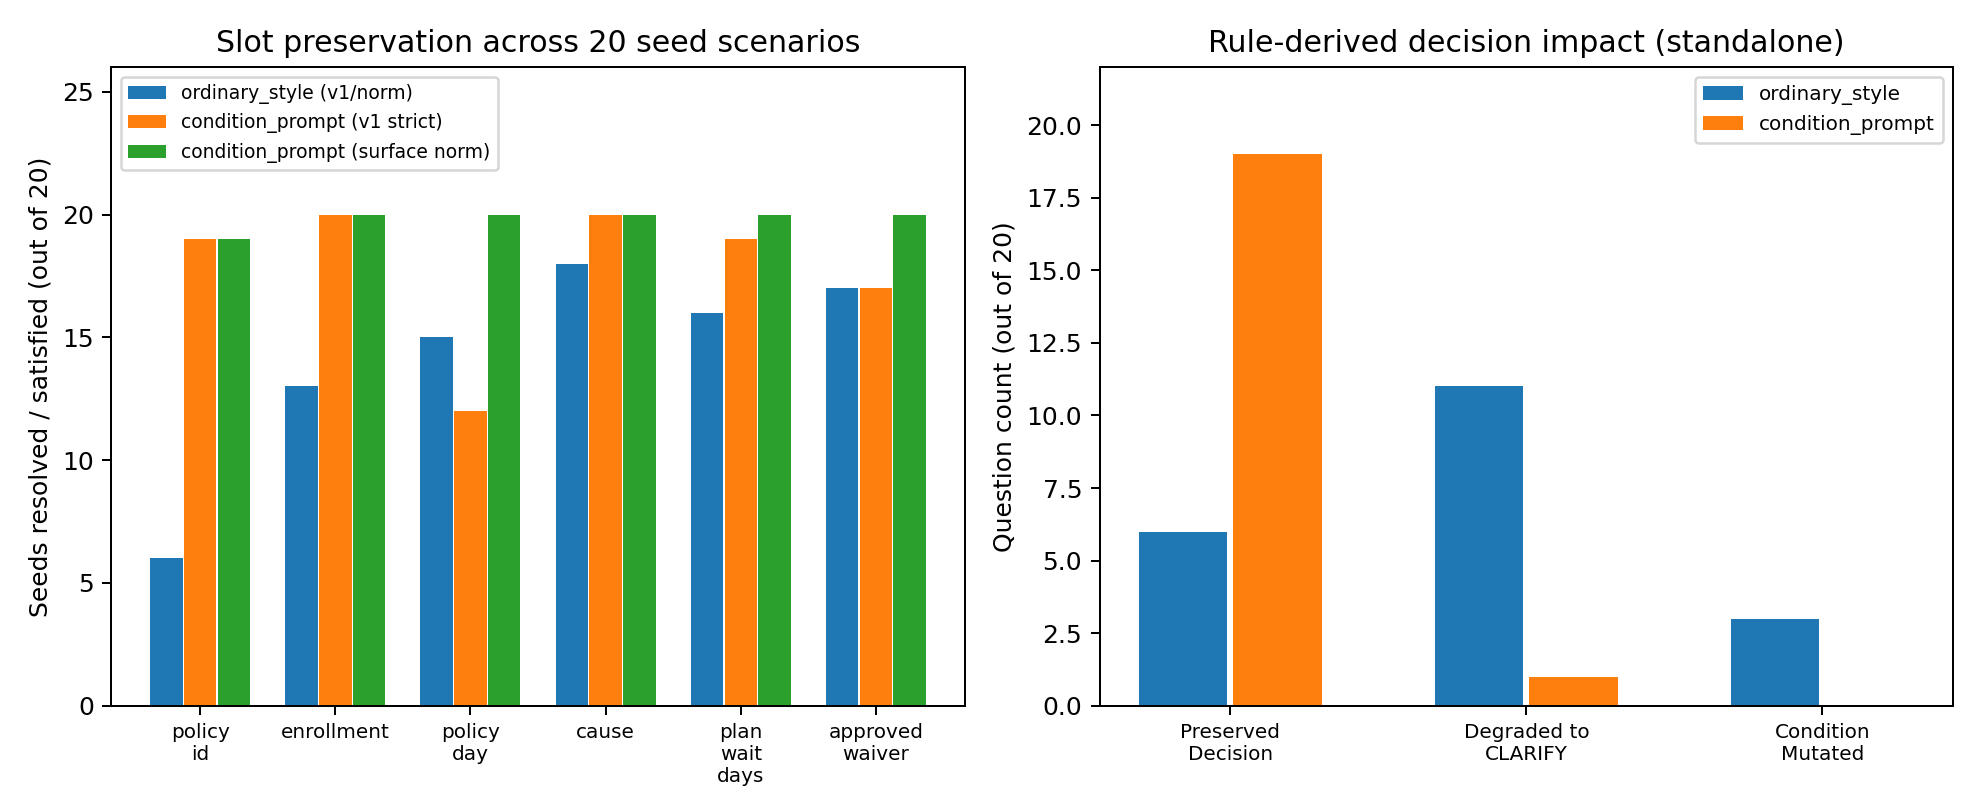
\includegraphics[width=\columnwidth]{figures/condition_preservation_comparison.png}
  \caption{Round~3 diagnostic comparison of slot retention and rule-decision outcomes under \texttt{ordinary\_style} vs.\ \texttt{condition\_prompt}.}
  \label{fig:round3}
\end{figure}

\subsection{Anatomy of Condition Drift Across Model Scales}
Table~\ref{tab:round3} and Figure~\ref{fig:round3} establish four key findings on vertical-domain query synthesis:

\paragraph{1. Syntactic Format Gates Are Blind Across All Scales.}
Across all three models, $100\%$ ($120/120$) of generated queries pass syntactic validation (\texttt{format\_valid}: single question mark, valid length, zero PII), yet $70\%\text{--}100\%$ of \texttt{ordinary\_style} queries lose standalone rule decidability.

\paragraph{2. Decomposing Scale-Dependent Hallucination vs.\ Scale-Invariant Pragmatic Omission.}
Comparing \texttt{1.5B}, \texttt{Qwen-Plus}, and \texttt{Qwen-Max} disentangles two distinct mechanisms of condition drift:
\begin{itemize}[leftmargin=*,nosep]
  \item \textbf{Scale-Dependent Value Hallucination}: Under \texttt{ordinary\_style}, the local \texttt{1.5B} model hallucinates numeric mutations in $15\%$ ($3/20$) of cases, rewriting ``生效第20天'' (Day~20) into ``生效后的第二天'' (Day~2), and collapses complementary CPIC Plan~C seeds (\texttt{condition-009} [7d wait $\rightarrow$ \texttt{WAIT\_NOT\_EXCLUDED}] and \texttt{condition-010} [25d wait $\rightarrow$ \texttt{WAIT\_EXCLUDED}]) into the exact same surface string: ``我是在网上看病花了钱，是第一次买这个保险，保单生效第10天了，因为不是意外病，想问一下这属于等待期吗？''. Scaling up to \texttt{Qwen-Plus} and \texttt{Qwen-Max} reduces numeric value mutations to \textbf{$0\%$ ($0/20$)}.
  \item \textbf{Scale-Invariant Pragmatic Omission}: However, scaling up model size \emph{worsens or fails to resolve} slot omission under \texttt{ordinary\_style}. Because larger models are better at mimicking brief, colloquial user phrasing, \texttt{Qwen-Plus} omits the formal product name in $100\%$ ($20/20$) of cases (yielding $0\%$ standalone decision preservation), while \texttt{Qwen-Max} omits product names in $50\%$ ($10/20$) of cases and paraphrases ``首次投保'' (first-time enrollment) into the legally ambiguous ``我刚买了…'' (``I just bought...'', which conflates first-time enrollment and annual renewal) in $30\%$ ($6/20$) of cases. Even when granting the true \texttt{policy\_id} via UI context, \texttt{ordinary\_style} preserves decisions in only $45\%$ (\texttt{Qwen-Plus}) and $50\%$ (\texttt{Qwen-Max}) of cases.
\end{itemize}

\paragraph{3. Universal Effectiveness of \texttt{condition\_prompt}.}
When prompted with explicit slot constraints (\texttt{condition\_prompt}), standalone rule-decision preservation jumps from $30\% \rightarrow 95\%$ on \texttt{1.5B}, from $0\% \rightarrow 95\%$ on \texttt{Qwen-Plus}, and from $20\% \rightarrow \mathbf{100\%}$ ($20/20$) on \texttt{Qwen-Max} (passing both \texttt{v1\_strict\_regex} and \texttt{v2\_synonym\_aware} without a single error). Top-1 clause retrieval over the 5-policy corpus similarly reaches $95\%\text{--}100\%$.

\subsection{Blinded Two-Rater Verification Protocol}
Because automated extractors can over-penalize natural paraphrases (\texttt{v1\_strict\_regex} exhibits $9/20$ false negatives on \texttt{1.5B} \texttt{condition\_prompt} outputs such as ``生效是第20天'' or ``同意免去等待期''), we package our evaluation suite into a blinded, randomized two-rater HTML annotation tool (\texttt{reviewer\_A.html} and \texttt{reviewer\_B.html} with automated Cohen's $\kappa$ scoring in \texttt{score\_annotations.py}).

\section{Practical Recommendations for RAG Cold-Start}
Our findings translate into three concrete guidelines for engineering teams cold-starting RAG systems in regulated verticals:
\begin{enumerate}[leftmargin=*,nosep]
  \item \textbf{Never Commit to Hybrid over Dense Retrieval on Uncalibrated Synthetic Benchmarks Alone}: Across both 1.5B and production cloud models, passage-conditioned synthetic queries inflate lexical overlap, systematically favoring BM25 and hybrid RRF even when pure dense retrieval wins on real user queries.
  \item \textbf{Use Candidate-Set Abstention under Small Calibration Budgets}: Collect $50\text{--}100$ group-disjoint real queries and apply paired-bootstrap candidate-set abstention rather than point selection or surface density reweighting.
  \item \textbf{Pair Larger Models with Explicit Slot Prompts and Counterexample Witnesses}: Scaling up LLM capacity eliminates numeric hallucinations but does not prevent conversational slot omission; always combine frontier models with explicit slot-constrained prompts (\texttt{condition\_prompt}) and verify decidability against single-field counterexamples.
\end{enumerate}

\section{Limitations}
First, while we validate our findings across three model tiers (\texttt{Qwen2.5-1.5B-Instruct}, \texttt{Qwen-Plus}, and \texttt{Qwen-Max}), all three belong to the Qwen instruction-tuned family; extending cross-family comparisons to GPT-4o and Claude-3.5 is a natural next step. Second, our Round~3 clause benchmark covers five representative Chinese health and medical policies ($80$ controlled cases and $120$ paired LLM rewrites); expanding coverage to life, property, and annuity clauses will further strengthen generalizability.

\bibliographystyle{plain}
\bibliography{references}

\end{document}
